% Loads of preamble stripped off - now located in mcstas.tex

%\newpage
\chapter{Polarization in McStas}
\label{c:polarization}
\begin{center}
\Large{P. Christiansen (Ris{\o})\\\today}
\end{center}

\section{Introduction}

In the current release of McStas there are components with polarization
capabilities. At the moment all such components should be understood as under
development as the amount of testing and debugging of these components is
small, and there are known problems.

Here, we shall report on what have been done so far.

We first describe the polarization vector and how it is related to the neutron
wave-function (section~\ref{sec:pol}) and then the physics of simple
components that we need in McStas is reviewed (section~\ref{sec:scat}). In the
last two sections the actual McStas polarization components are first
described (section~\ref{sec:new}) and a list of test instruments in McStas is
given (section~\ref{sec:test}).

We rely heavily on the books~\cite{lovesey84,gavin} for the physics where
the detailed calculations can be found.

The notation used here (and in~\cite{gavin}) is $P$ (scalar), $\PB$
(vector), $\tP$ (unit-vector), $\sigmaH$ (operator), and $\sigmao$
(vector of operators).

\section{The Polarization Vector}
\label{sec:pol}

The spin of the neutron is represented by an operator $\so$ for which only a
single component can be measured at one time. Each single measurement will
give a value $\pm 1/2$, but if we could make a large number of measurements on
the same neutron state, in each of the three axis directions, and then make
the average we get $\langle \so \rangle$. The polarization vector, $\PB$, is
then defined as:
\begin{equation}
  \label{eq:pol_single}
  \PB = \frac{\langle \so \rangle}{s},
\end{equation}
so that $-1 \leq |\PB| \leq +1$

For a neutron beam which contains $N$ neutrons, each with a
polarization $\PB_i$, the beam polarization is defined as:
\begin{equation}
  \label{eq:pol_beam}
  \PB = \frac{\sum_i \PB_i}{N}.
\end{equation}

If we have one common quantization direction (e.g. a magnetic field
direction) each neutron will either be spin up, $\uparrow$, or spin down,
$\downarrow$, and the polarization can be expressed as:

\begin{equation}
  \label{eq:pol}
  P = \frac{\nup-\nd}{\nup+\nd},
\end{equation}

where $\nu$ ($\nd$) is the number of neutrons with spin up
(down).

For a given neutron the probability of the neutron being spin up, $\Pu$, is:

\begin{equation}
  \label{eq:prob_spinup}
  \Pu = \frac{\nup}{\nup+\nd} = \frac{\nup + (\nd-\nd)/2}{\nup+\nd}
  = \frac{1+P}{2},
\end{equation}

and $\Pd = 1-\Pu = (1-P)/2$.

The expectation value of the 'spin' operator, $\sigmao$, which can be
expressed by the Pauli matrices, is the polarization vector $\PB$, $\PB =
\langle \sigmao \rangle \equiv \langle \chi | \sigmao | \chi \rangle$.  The
most general form of the spin wave-function $\chi$ for a neutron (spin 1/2)
is:

\begin{equation}
  \label{eq:neutron_wave}
  \chi = a\chi_\uparrow + b\chi_\downarrow,
\end{equation}

where $\chi_\uparrow$ and $\chi_\downarrow$ are eigenfunction of
$\hat{\sigma}^z$, and the complex coefficients $a$ and $b$ satisfy
$|a|^2 + |b|^2 = 1$.

By calculation we find:
\begin{eqnarray}
P_x & = & \langle \chi | \sigmaH_x | \chi \rangle
= 2 \text{Re}(a^\ast b) \\
P_y & = & \langle \chi | \sigmaH_y | \chi \rangle
= 2 \text{Im}(a^\ast b) \\
P_z & = & \langle \chi | \sigmaH_z | \chi \rangle
= |a|^2-|b|^2
\end{eqnarray}

This shows the relation of the polarization vector to the neutron wave
function.

The neutron magnetic moment operator can be expressed in terms of $\sigmao$,
as:
\begin{equation}
  \label{eq:magnetic}
  \muno = \mu_n \sigmao,
\end{equation}
which, as shown above, is related to the polarization vector.  \\

In our simulation we represent the polarization by the vector $\SB = (s_x,
s_y, s_z)$ which is propagated through the different components so it has the
correct relative orientation in each component. The probability for the spin
to be parallel a given direction $\mathbf{n}$ is then:

 \begin{equation}
   \label{eq:probmcstas}
   P(\uparrow|\nB) = \frac{1+\nB \cdot \SB}{2}.
 \end{equation}

This equation (from~\cite{pol_seeger}) is easy to understand. The
average spin along $\nB$ is $\nB \cdot \SB$ and the probability then
follows from Eq.~\ref{eq:prob_spinup}.

For an unpolarized beam, $\mathbf{S} = \mathbf{0}$ and all directions
are equally probable (50~\%).

Note that in our approach we do not decide if the neutron is up or down after
a given component, but instead keep track of as much information for as long
as possible.

In the following we will use $\PB$ to denote the polarization
vector. The most important variables used are:

\begin{tabular}{ll}

  $\Q$  & Scattering vector. \\
  $\PB$  & Polarization before a component (ingoing). \\
  $\PB_\perp$  & Polarization perpendicular to scattering vector,
  $\PB_\perp = \tQ \times (\PB \times \tQ$). \\
  $\PB'$ & Polarization after a component (outgoing). \\
  $\tN$ & Unit vector in direction of atomic spin ($\tN \cdot \tilde{\BB} = -1$ for a ferromagnet). \\
  $\FN$ & Unit cell nuclear structure factor. \\
  $\FM$ & Unit cell magnetic structure factor. \\
\end{tabular}
\\

The unit cell nuclear structure factor is defined as:

\begin{equation}
  \FN = \sum_\dB
  \exp(i\Q \cdot \dB)\overline{b}_d,
\end{equation}

where the $\dB$ is the position of the d'th atom within the unit cell,
and $\overline{b}_d$ is the average of $b_d$. In the simple case of a
single atom Bravais crystal one finds $\FN = \overline{b}$.

The unit cell magnetic structure factor is useful when the atoms in
the crystal only have spin orbital angular momentum, and simple when
the magnet is saturated (all spins are parallel or anti-parallel to
\emph{one} direction, $\sigma_d=\pm1$). It is then given as:

\begin{equation}
  \FM =
  \gamma_n r_0 \sum_\dB \exp(i\Q \cdot \dB)\frac{1}{2}g_d F_d(\Q)\langle
  \hat{S}_d\rangle \sigma_d,
\end{equation}

where $r_0=\frac{\mu_0}{4\pi}\frac{e^2}{m_e} = 2.818 \times 10^{-15}$m, $g=2$ is the
Land{\'e} splitting factor, and $F_d(\Q)$ is the magnetic form factor, which
is the Fourier transform of the magnetization density (normalized so that
$F_d(0) = 1$), and $\langle \hat{S}_d\rangle$ is the thermal average of the
ordered atomic spin.

In the following the Debye-Weller factor ($\exp(-W_d)$) have been ignored in
all cross sections.

\subsection{Example: Magnetic fields}

The magnetic moment operator of the neutron is $\muno = \gamma_n \so$, where
$\gamma_n = 2 \mu_n = -3.826$ is the gyromagnetic ratio (spin and magnetic
moment is anti-parallel as for an electron)~\footnote{Note that if we had used
S (with values $S=\pm 1$) to define $\gamma_n$ we would get $\gamma_n =
-1.913$ which is also commonly used.}

A magnetic field, $\BB$, will exert a torque, $\tauB = d\sB/dt = (1/\gamma_n)d\muB/dt$, on the neutron magnetic moment:

\begin{equation}
  \label{eq:torque}
  \frac{1}{\gamma_n} \frac{d\muB}{dt} = \muB \times \BB
\end{equation}

The magnetic moment $\mu$ can be related to the polarization as $\muB
= \gamma_n \PB/2$, and inserting in Eq.~\ref{eq:torque} we find:

\begin{equation}
  \label{eq:pol_magnetic}
  \frac{d\PB}{dt} = \gamma_n \PB \times \BB
\end{equation}

In the simple case where $\BB = (0, 0, B)$, we find the solution
(\cite{gavin} p.~18) :

\begin{eqnarray}
  \nonumber
  P_X(t) & = & \cos(\omega_L t) P_X(0) - \sin(\omega_L t) P_Y(0) \\
  \label{eq:precession}
  P_Y(t) & = & \sin(\omega_L t) P_X(0) + \cos(\omega_L t) P_Y(0) \\
  \nonumber
  P_Z(t) & = & P_Z(0),
\end{eqnarray}

where $\omega_L = -\gamma_n B/\hbar$ is the Larmor frequency.\\

\begin{quote}
  The equations above was checked against the equations in the ``polarimetrie
  neutronique'' notes by Francis Tasset and found to be consistent. There can
  be sign differences between different publications depending on whether they
  use a right-handed (like e.g. McStas) or a left-handed (like e.g. NISP)
  coordinate system.
\end{quote}

\section{Polarized Neutron Scattering}
\label{sec:scat}

First we will give a short introduction to how calculations are done
and then quote some results which are important for implementing the
first McStas components.

All the potentials (nuclear, magnetic, and electric) we will be interested in
can be written on the form:
\begin{equation}
  \label{eq:general_pot}
  \hat{v} = \betao + \alphao \cdot \sigmao
\end{equation}

The first term does not affect the spin, while the second term can
change the spin. Let us just remind here that:

\begin{equation}
  \label{eq:pauli_rules}
  \begin{matrix}
    \sigmaH_x \chiU = \chiD, &
    \sigmaH_y \chiU = i\chiD, &
    \sigmaH_z \chiU = \chiU, \\
    \sigmaH_x \chiD = \chiU, &
    \sigmaH_y \chiD = -i\chiU, &
    \sigmaH_z \chiD = -\chiD.
  \end{matrix}
\end{equation}

So that the interaction proportional to $\sigmaH_x$ and $\sigmaH_y$
results in spin flips, while the interactions with $\sigmaH_z$
conserves the spin.

It turns out to be smart to define a density matrix operator:
\begin{equation}
  \rhoo = \chi \chi^\dagger =
  \left( \begin{matrix}
    |a|^2 & ab^\ast \\
    ba^\ast & |b|^2
  \end{matrix} \right)
  = \frac{1}{2}({\cal I}+\PB \cdot \sigmao),
\end{equation}
where $\chi$ is the neutron wave function (Eq.~\ref{eq:neutron_wave}),
and ${\cal I}$ is the unit matrix.

Using the density matrix the elastic cross section can be written as
(\cite{lovesey84}, Eq.~10.31):
\begin{equation}
  \label{eq:master_sigma}
  \frac{d\sigma}{d\Omega} = \text{Tr} \rhoo \hat{v}^\dagger \hat{v}
  = \sum_{\lambda, \lambda'} p_\lambda \text{Tr} \rhoo
  \langle \lambda | \hat{V}^\dagger(\Q) | \lambda' \rangle
  \langle \lambda' | \hat{V}(\Q) | \lambda \rangle
  \delta(E_\lambda - E_{\lambda'}),
\end{equation}

where $\hat{V}$ is the interaction potential and it is understood that
the trace is to be taken with respect only to the neutron spin
coordinates. The outgoing polarization is given as:
\begin{equation}
  \label{eq:master_pol}
  \PB' \frac{d\sigma}{d\Omega} =
  \text{Tr} \rhoo \hat{v}^\dagger \sigmao \hat{v}
  = \sum_{\lambda, \lambda'} p_\lambda \text{Tr} \rhoo
  \langle \lambda | \hat{V}^\dagger(\Q) | \lambda' \rangle
  \sigmao
  \langle \lambda' | \hat{V}(\Q) | \lambda \rangle
  \delta(E_\lambda - E_{\lambda'})
\end{equation}

Inserting Eq.~\ref{eq:general_pot} in Eq.~\ref{eq:master_sigma} and
Eq.~\ref{eq:master_pol} results in the two master equations for
polarized neutron scattering:

\begin{equation}
  \label{eq:general_sigma}
  \text{Tr} \rhoo \hat{v}^\dagger \hat{v} =
  \alphao^\dagger \cdot \alphao + \betao^\dagger \betao+
  \betao^\dagger (\alphao \cdot \PB) +
  (\alphao^\dagger \cdot \PB) \betao +
  i\PB \cdot (\alphao^\dagger \times \alphao),
\end{equation}

and

\begin{equation}
  \label{eq:general_pol}
  \text{Tr} \rhoo \hat{v}^\dagger \sigmao \hat{v} =
  \betao^\dagger \alphao
  + \alphao^\dagger \betao
  + \betao^\dagger \betao \PB
  + \alphao^\dagger (\alphao \cdot \PB)
  + (\alphao^\dagger \cdot \PB) \alphao
  - \PB (\alphao^\dagger \cdot \alphao)
  - i \alphao^\dagger \times \alphao
  + i \betao^\dagger (\alphao \times \PB)
  + i (\PB \times \alphao^\dagger) \betao.
\end{equation}

Based on these two equations and the interaction potentials all the
results presented in the following are derived in~\cite{lovesey84}.

\subsection{Example: Nuclear scattering}

The nuclear scattering potential for a crystal is:
\begin{equation}
  \label{eq:nuclear_pot}
  \hat{V}_N(\Q) = \sum_{\lB,\dB} \exp(i\Q \cdot \RB_{ld})(A_{ld} +
  \frac{1}{2} B_{ld} \sigmao \cdot \Io_{ld}),
\end{equation}

so that

\begin{eqnarray}
  \label{eq:ab_nuclear}
  \alphao & = &
  \sum_{\lB,\dB} \exp(i\Q \cdot \RB_{ld}) \frac{1}{2} B_{ld} \Io_{ld} \\
  \betao & = &
  \sum_{\lB,\dB} \exp(i\Q \cdot \RB_{ld}) A_{ld},
\end{eqnarray}

where $\Io$ is the nuclear spin operator and the constants $A$ and $B$
are related to the nuclear scattering lengths $b^+$ and $b^-$ as
$A=((I+1)b^++Ib^-)/(2I+1)$ and $B=(b^++b^-)/(2I+1)$.

To calculate the polarization cross section and outgoing polarization
we have to average over the nuclear spin (which we assume is random
oriented), so that terms linear in $\alphao$ (three last terms in
Eq.~\ref{eq:general_sigma}) disappears. The scattering cross section
ends up being (see~\cite{lovesey84} p.~159):

\begin{equation}
  \label{eq:nuclear_sigma}
  \frac{d\sigma}{d\Omega}  =
  \sum_{\lB, \dB, \lB', \dB'} \exp(i \Q \cdot (\RB_{ld}-\RB_{l'd'}))
  (\madsq + \delta_{\lB,\lB'}\delta_{\dB,\dB'}[\sqmad - \madsq
  + \frac{1}{4}\bd])
\end{equation}

where the first term is the coherent cross-section and the second term is the
site-incoherent cross-section. Both terms are independent of $\PB$ as expected
for a system without a preferred internal direction.

The polarization in the final state is:

\begin{equation}
  \label{eq:nuclear_pol}
  \PB' \frac{d\sigma}{d\Omega}  =
  \sum_{\lB, \dB, \lB', \dB'} \exp(i \Q \cdot (\RB_{ld}-\RB_{l'd'}))
  \PB' (\madsq + \delta_{\lB,\lB'}\delta_{\dB,\dB'}[\sqmad - \madsq
  - \frac{1}{12}\bd])
\end{equation}

Comparing Eq.~\ref{eq:nuclear_sigma} and Eq.~\ref{eq:nuclear_pol} we
find that: 1) The nuclear coherent polarization is the same as the
initial polarization. 2) The same is true for the incoherent
scattering due to the random isotope distribution. 3) The nuclear
incoherent scattering due to the random nuclear spin orientations has
polarization $\PB' = -1/3 \PB$ (for a random nuclear spin the
associated Pauli matrix will 2/3 of the time point in the direction of
$\sigmaH_x$ and $\sigmaH_y$ which according to
Eq.~\ref{eq:pauli_rules} flips the spin). \\

For Vanadium, where there is only one isotope and coherent scattering
is negligible, we find $\PB' = -1/3\PB$. There is however one
catch. If the probability for multiple scattering is large one has to
take into account that after two scattering one has: $\PB'(2) =
1/9\PB$, and so forth. The average polarization after a thick vanadium
target is therefore a sum of different contributions.

\subsection{Example: Polarizing Monochromator and Guides}
\label{sub:mono}

\begin{figure}[htbp]
  \begin{center}
    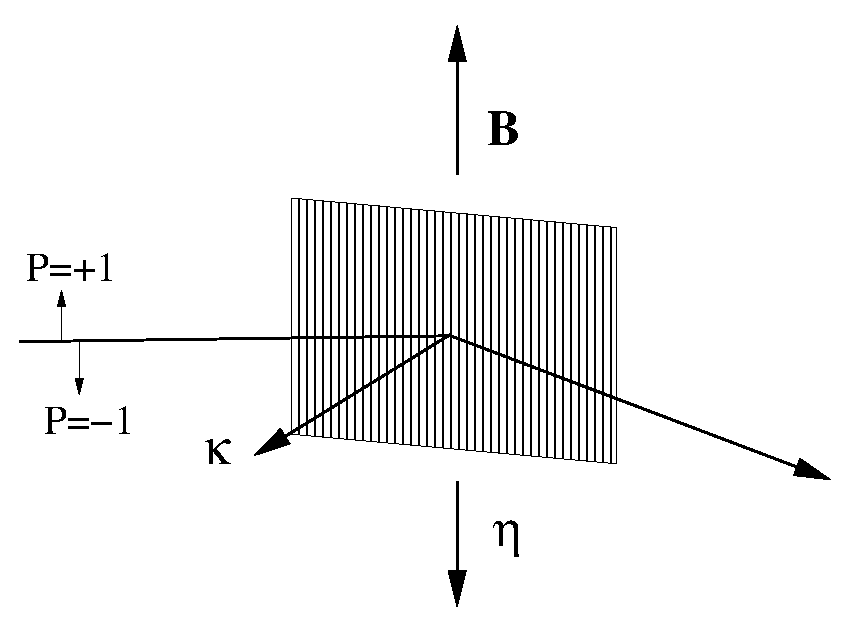
\includegraphics[keepaspectratio,
    width=0.7\columnwidth]{figures/monochromator_pol}
    \caption{Principle and geometry of a polarizing monochromator.}
    \label{fig:mono_princip}
  \end{center}
\end{figure}

In a polarized monochromator and polarizing guides we have a ferromagnetic
crystal in an external magnetic field. The scattering potential is now both
nuclear (no internal direction) and magnetic (internal direction), so in
general the outgoing polarization can be quite complex. However, as
illustrated in Figure~\ref{fig:mono_princip}, the typical setup has many
geometrical constraints: $\tN \cdot \tQ = 0$, $\tN \cdot \PB_\perp = \tN \cdot
\PB$, and $\Q \times (\tN \times \Q) = \tN$, which simplifies the problem.

In~\cite{lovesey84} the calculation for a centrosymmetric ferromagnetic
crystal is done, and inserting the constraints above one finds
(\cite{lovesey84}, Eq.~10.96 and Eq.~10.110):

\begin{eqnarray}
  \label{eq:mono_sigma}
  d\sigma/d\Omega & = & \FN^2 + 2\FN\FM (\PB \cdot \tN) + \FM^2\\
  \label{eq:mono_pol}
  \PB' d\sigma/d\Omega & =
  & \PB [\FN^2 - \FM^2] + \tN [2\FN\FM + 2(\tN \cdot \PB)\FM^2]
\end{eqnarray}

\begin{quote}
  NB! Note that in~\cite{gavin} Eq.~2.2.25 there is a minus in front of the
  second term in Eq.~\ref{eq:mono_sigma}. We have not been able to understand
  this discrepancy, which is probably due to notation. Most other authors
  agree with the minus in front of the second term (e.g. Squires and Francis
  Tasset).
\end{quote}

For a beam which is initially unpolarized we find the outgoing
polarization to be:
\begin{equation}
  \PB' = \frac{\tN 2\FN \FM}{d\sigma/d\Omega}
  = \frac{2\FN\FM}{\FN^2 + \FM^2} \tN,
\end{equation}

so that the beam is fully polarized along $\tN$ if $\FN = \pm \FM$. \\

What we use to characterize the polarizing monochromator in practice
is not $\FN$ and $\FM$, but instead the reflection probabilities $\Ru$
and $\Rd$ (for the reflection of interest).

If we assume that the reflection probabilities are directly proportional to
the cross sections (with proportionality constant $k$), i.e., $\Ru = k
d\sigma/d\Omega(\PB=+\tN)$ and $\Rd = k d\sigma/d\Omega(\PB=-\tN)$ then we can
use Eq.~\ref{eq:mono_sigma} to determine $\FN$ and $\FM$:

\begin{eqnarray}
  \label{eq:mono_up}
  \Ru & = & k (\FN + \FM)^2,\\
  \label{eq:mono_down}
  \Rd & = & k (\FN - \FM)^2.
\end{eqnarray}

The values of $\sqrt{k}\FN$ and $\sqrt{k}\FM$ are then between -1 and +1 and
unit less like the reflection probabilities. In the following we ignore $k$ and
just talk about $\FN$ and $\FM$.

In principle there are four solutions for $\FN$ and $\FM$, so in the code we
currently choose the values where $\FN + \FM = +\sqrt{\Ru}$ and $\FN - \FM =
+\sqrt{\Rd}$ (so that $\FN>0$ and $\FN>\FM$). We then find:

\begin{eqnarray}
  \label{eq:mono_nuc}
  \FN & = & \frac{\sqrt{\Ru} + \sqrt{\Rd}}{2},\\
  \label{eq:mono_mag}
  \FM & = & \frac{\sqrt{\Ru} - \sqrt{\Rd}}{2}.
\end{eqnarray}

When $\FN$ and $\FM$ are determined from these equations,
Eq.~\ref{eq:mono_sigma} and Eq.~\ref{eq:mono_pol} can easily be used to handle
any situation.

This solution is both used for monochromators and guides.

It is not clear that this solution is correct. If we make a simple example
with $\Ru = 1$ and $\Rd = 0.25$ then we could in principle have four
solutions, but let us just quote the two where $\FN$ is positive since the
last two are found by inserting a minus before all the solutions and this does
not change the physics. The two solutions are $\FN = 0.75, \FM=0.25$ and $\FM
= 0.75, \FN=0.25$. All solutions gives the same cross section, but if the
incoming beam is polarized (and only then) the outgoing beam will have two
different polarization values, since $\PB [\FN^2 - \FM^2]$ and $\tN 2(\tN
\cdot \PB)\FM^2$ are different for the two solutions. It seems that one needs
some additional information to choose between the two solutions.

\begin{quote}
  NB! The simplifying geometry shown in Figure~\ref{fig:mono_princip} only
  applies for the sides of the guide wall and not the top and bottom (assuming
  that the magnetizing field is pointing up or down), so there another set of
  equations should really be used.
\end{quote}

The same physics could also be used for a polarizing powder or single crystal
sample if $\FN$ and $\FM$ can be calculated with some other program, but one
would have to use the general form of Eq.~\ref{eq:mono_sigma} and
Eq.~\ref{eq:mono_pol} without the simplifying geometrical constraints for
monochromators and guides.

\section{New McStas Components}
\label{sec:new}

The components written so far can be divided into four groups:
\begin{itemize}
\item \textbf{Polarizers:} Components used to make the beam polarized.
\item \textbf{Monitors:} Unphysical detectors that can measure the polarization
of the neutrons.
\item \textbf{Magnetic fields:} Components used to handle magnetic fields.
\item \textbf{Samples:} Samples that affects the polarization.
\end{itemize}

\subsection{Polarizers}

Some of the most common ways of polarizing a beam have been
implemented.

\begin{itemize}
\item \textbf{Set\_pol:} This unphysical component can be used in two
ways. Either to hard code the polarization to the vector $(px, py, pz)$
or when randomOn!=0 to set the polarization vector to a random vector
on the unit sphere.\\

\item \textbf{Monochromator\_pol:} A monochromator that only does the $n=1$
  reflection. For each neutron it calculates the wavelength which would give
  Bragg reflection, $\lambda_\text{Bragg}$, and it then calculates, based on
  one mosaicity and one d-spread, the reflection probability given the neutrons
  actual $\lambda$.  The reflection probability is a Gaussian in $\Delta
  \lambda = \lambda - \lambda_\text{Bragg}$, with the peak reflectivity and
  polarization calculated as described in section~\ref{sub:mono}.

  \begin{quote}
    NB! Note that this monochromator reflects the neutrons billiard-like. In
    \textbf{Monochromator\_flat} the mosaicity of the reflecting crystal is
    taken into account, but the d-spread is not taken into account. One should
    implement d-spread and mosaicity in a way similar to what is done in
    \textbf{Single crystal}.
  \end{quote}

\item \textbf{Pol\_mirror:} Plane with a reflection probability for up
and down. There are 3 options: always reflect, always transmit, or
random select transmit/reflect.

\begin{quote}
  NB! Note that at the moment the plane only reflects from one side (because
  it uses PROP\_Z0.
\end{quote}

\item \textbf{Pol\_bender:} Curved guide with the possibilities to
  insert multiple slits, and have the end gap parallel to the entrance
  or following the guide angle. It is possible to select different
  coatings (mirror parameters) for each of the four sides.\\

\item \textbf{Pol\_guide\_vmirror:} Straight guide with non-polarizing
  coatings with two polarizing super mirrors sitting in a V shape
  inside. \\
\end{itemize}

Note that for all the polarizing guides it is possible to define analytical
functions or use tables for the up and down reflectivity descriptions.

\subsection{Detectors}

\begin{itemize}
\item \textbf{Pol\_monitor:} One defines a vector $\mathbf{m} = (mx,
  my, mz)$ for the monitor and measures the projection of the spin
  along this vector i.e. $\mathbf{m} \cdot \mathbf{S}$.\\

\item \textbf{PolLambda\_monitor:} Measures the projection of the
  spin along the defined vector $\mathbf{m}$ (see
  \textbf{Pol\_monitor}) as a function of the wavelength $\lambda$.

\item \textbf{MeanPolLambda\_monitor:} Measures the \emph{average}
  projection of the spin along the defined vector $\mathbf{m}$ (see
  \textbf{Pol\_monitor}) as a function of the wavelength $\lambda$.

  \begin{quote}
    NB! currently the error on the mean is shown ($\sigma/\sqrt(N)$), but it
    might make more sense to show the spread ($\sigma$).
  \end{quote}
\end{itemize}

\subsection{Magnetic fields}

Much inspiration for the components and the tests have been found
in~\cite{pol_seeger}.

\begin{itemize}
\item \textbf{Pol\_constBfield:} A rectangular box with a constant magnetic
  field in the y-direction. The x- and z-components of the spin precess with
  the Larmor frequency $\omega_L$. It is possible to define the field in terms
  of a wavelength so that the spin will precess 180 degrees for the given
  wavelength. The component can be rotated to have the field along another
  axis. \\

\item \textbf{Pol\_simpleBfield:} The first attempt at a component for
  handling general magnetic fields. It is a concentric component where you
  define a start and stop component for each field, but this allows other
  components, e.g. monitors, to be put inside the field. The component
  overloads the propagation routines so that numerical spin propagation is
  done for analytical magnetic fields.

  \begin{quote}
    NB! At the moment both components does not really check the boundaries of
    the field on the sides, but merely assumes that the field starts at the
    entrance plane and stops at the exit plane.

    Also, some optimization remains for the numerical component and it would
    be nice to support tabulated magnetic field files. However, the framework
    developed for \textbf{Pol\_simpleBfield} is very general and should
    easily facilitate these changes.
  \end{quote}

\end{itemize}


\subsection{Samples}

\begin{itemize}
\item \textbf{V\_sample:} Modified the sample so that the scattered
  neutron has $\PB' = -1/3\PB$. Note that this component does not
  handle multiple scattering, so this approach is correct. If the
  components handled multiple scattering the polarization should be
  set to $\PB' = (-1/3)^n\PB$, where $n$ is the number of
  scatterings.\\
\end{itemize}


\section{Tests With New Components}
\label{sec:test}

All the test instruments can be found in the McStas examples folder
(go to ``Neutron site/tests'' in mcgui).

There are basically two kind of tests. The first kind of tests shows
that the polarizing component can reproduce the same results as a
similar non-polarizing component:
\begin{itemize}
\item \textit{Test\_Monochromators.instr} : Intercomparison of
  \textbf{Monochromator\_flat} and \textbf{Monochromator\_pol}.
\item \textit{Test\_Pol\_Bender\_Vs\_Guide\_Curved.instr} : Intercomparison of
  \textbf{Guide\_curved} and \textbf{Pol\_bender}.
\end{itemize}

The second type of test illustrates the polarizing capabilities of the
component:
\begin{itemize}
\item \textit{Test\_Magnetic\_Constant.instr} : Constant magnetic field.
\item \textit{Test\_Magnetic\_Majorana.instr} : Linearly decreasing field with
  small transverse component.
\item \textit{Test\_Magnetic\_Rotation.instr} : Rotating magnetic field.
\item \textit{Test\_Magnetic\_Userdefined.instr} : Example of how to make a
  user defined analytic magnetic field that can also depend on time.
\item \textit{Test\_Pol\_Bender.instr} : Illustrates beam polarization with
  the \textbf{Pol\_bender}.
\item \textit{Test\_Pol\_Set.instr} : Tests \textbf{Pol\_set}.
\item \textit{Test\_Pol\_Guide\_Vmirror.instr} : Illustrates beam polarization
  with the \textbf{Pol\_guide\_vmirror}.
\item \textit{Test\_Pol\_Mirror.instr} : Illustrates beam polarization
  with the \textbf{Pol\_mirror}.
\item \textit{Test\_Pol\_TripleAxis.instr} : An example of a triple axis
  spectrometer with polarizing monochromators, a vanadium sample, and a spin
  flipper.
\end{itemize}

